\documentclass{physlab}

\begin{document}
\begin{titlepage}
\center % Center everything on the page
 
%----------------------------------------------------------------------------------------
%	HEADING SECTIONS
%----------------------------------------------------------------------------------------

\textsc{\LARGE Московский\\[-0.2cm]Физико-Технический Институт\\[0.1cm]\large (государственный университет)}\\[1.5cm] % Name of your university/college
\textsc{\Large Кафедра общей физики}\\[0.1cm] % Major heading such as course name
\textsc{\large Лабораторная работа № 5.1}\\[0.5cm] % Minor heading such as course title

%----------------------------------------------------------------------------------------
%	TITLE SECTION
%----------------------------------------------------------------------------------------

\HRule
\\
{\huge \bfseries Измерение коэффициента ослабления \\[-3mm]
потока $\gamma$-лучей в веществе \\[3mm]
и определение их энергии}
\\[0.3cm] % Title of your document
\HRule
\\[1.5cm]


 
%----------------------------------------------------------------------------------------
%	AUTHOR SECTION
%----------------------------------------------------------------------------------------

\begin{minipage}[t]{0.48\textwidth}
	\begin{flushleft} \large
		\textsf{Студент}
		
		Ришат \textsc{Исхаков} \\[-0.15cm]
		512 группа

	\end{flushleft}
\end{minipage}
\hfill
\begin{minipage}[t]{0.48\textwidth}
	\begin{flushright} \large
		\textsf{Преподаватель}		
		
		Лев Владиславович \\[-0.15cm]
		\textsc{Инжечик} 

	\end{flushright}
\end{minipage}

\begin{bottompar}
	\begin{center}
		
\includegraphics[width = 80 mm]{logo.jpg}
	\end{center}
	\today

\end{bottompar}
\vfill % Fill the rest of the page with whitespace

\end{titlepage}

\paragraph{Цель работы:} Определить энергию $\gamma$-квантов неизвестного радиоактивного препарата после предварительной калибровки спектрометра по $\gamma$-излучению $^{60}Co$.

\section{Теория}
Принцип действия спектрометра состоит в следующем:
\begin{enumerate}
    \item $\gamma$-кванты от исследуемого источника коллимируются свинцовым коллиматором и попадают в сцинтиллятор~---~кристалл йодистого натрия, активизированного таллием (NaI(TI)).
    \item Попавшие в сцинтиллятор $\gamma$-кванты взаимодействуют с атомами, выбивая из них электроны. При больших энергиях возможно образование электрон-позитронных пар. Возбужденные атомы высвечиваются, испуская электро-магнитное излучение.
    \item Часть образовавшихся фотонов, пройдя через сцинтяллятор, попадает на катод фотоэлектронного умножителя и в результате фотоэффекта выбивает из него медленные электроны. Эти электроны ускоряются полем умножителя и вырывают с поверхности первого динода, вторичные электроны, которые ускоряются полем по направлению ко второму диноду и т.д. Многократное повторение этого процесса позволяет получить большой коэффициент умножения.
\end{enumerate}  

Hello, my name is Rishat

Энергия конверсионного электрона:
\[ T_e = E_\gamma - W_K,\] 
где $W_K$~---~энергия нужная для ионизации K-оболочки атома.

Наибольшая энергия, которая может быть передана электрону (наименьшая равна нулю):
\[ (T_e)_{max} = \hbar \omega \dfrac{2 \alpha}{1 + 2 \alpha}, \] где $\alpha = \hbar \omega / (mc^2)$.

Если энергия $\gamma$-кванта $> 2mc^2$, то возможно образование электрон-позитронной пары в поле ядра. В таком случае сумма кинетических энергий электрона и позитрона равна:
\[ T_{e^-} + T_{e^+} = \hbar \omega - 2mc^2.\]
Идентификацию $\gamma$-линий будем проводить по пикам полного поглощения (в нашем случае ширина аппаратурная, а не истинная). Ширину пика будем характеризовать энергетическим разрешением прибора:
\[R = \dfrac{\delta}{E} \cdot 100 \% ,\] где $\delta$~---~ширина пика полного поглощения на половине высоты, $E$~---~энергия регистрируемого $\gamma$-излучения.

\section{Ход работы}
	
Сначала проградуируем спектрометр по $\gamma$-излучению $^{60}Co$, испускающего $\gamma$-линии с энергиями $E_1 = 1.17~\M \eV$ и $E_2 = 1.33~\M \eV$. Затем определим энергии $\gamma$-квантов неизвестного препарата.

\begin{table}[H]
\centering
\caption{Результаты измерения для $^{60}Co$}
\resizebox{\textwidth}{!}{%
\begin{tabular}{|c|c|c|c|c|c|c|c|c|c|c|c|c|c|c|c|c|}
\hline
$V_\text{порог}$ & 10 & 9.9 & 9.8 & 9.7 & 9.6 & 9.5 & 9.4 & 9.3 & 9.2 & 9.1 & 9  & 8.9 & 8.8 & 8.7   \\ \hline
N                & 3  & 10  & 14  & 21  & 10  & 15  & 24  & 26  & 44  & 47  & 33 & 39  & 41  & 34    \\ \hline
$V_\text{порог}$ & 8.6 & 8.5 & 8.4 & 8.3 & 8.2 & 8.1 & 8   & 7.9  & 7.8  & 7.7  & 7.6  & 7.5  & 7.4  & 7.3      \\ \hline
N          & 75  & 85  & 78  & 24  & 273 & 478 & 791 & 1307 & 1699 & 1901 & 1832 & 1542 & 1275 & 1038   \\ \hline
$V_\text{порог}$ & 7.2 & 7.1 & 7    & 6.9 & 6.8  & 6.7  & 6.6  & 6.5  & 6.4  & 6.3  & 6.2  & 6.1  & 6    & 5.9      \\ \hline
N & 908 & 1313 & 1910 & 2300 & 2678 & 2854 & 2889 & 2345 & 2010 & 1751 & 1591 & 1569 & 1385 & 1505   \\ \hline
$V_\text{порог}$ & 5.8  & 5.7  & 5.6 & 5.5  & 5.4  & 5.3 & 5.2  & 5.1  & 5    & 4.9  & 4.8  & 4.7  & 4.6  & 4.5      \\ \hline
N & 1581 & 1694 & 1733 & 1919 & 2184 & 2197 & 2286 & 2244 & 2434 & 2392 & 2327 & 2434 & 2207 & 2273   \\ \hline
$V_\text{порог}$ & 4.4  & 4.3  & 4.2  & 4.1 & 4    & 3.9  & 3.8  & 3.7 & 3.6  & 3.5  & 3.4  & 3.3  & 3.2  & 3.1  \\ \hline
N  & 2223 & 2104 & 2268 & 2250 & 2219 & 2190 & 2281 & 2192 & 2261 & 2243 & 2275 & 2174 & 2194 & 2214 \\ \hline
\end{tabular}}
\end{table}

\begin{table}[H]
\centering
\caption{Результаты измерения для неизвестного вещества}
\resizebox{\textwidth}{!}{%
\begin{tabular}{|c|c|c|c|c|c|c|c|c|c|c|c|c|c|c|c|c|}
\hline
$V_\text{порог}$ & 10 & 9.9 & 9.8 & 9.7 & 9.6 & 9.5 & 9.4 & 9.3 & 9.2 & 9.1 & 9 & 8.9 & 8.8 & 8.7 \\ \hline
N & 1  & 7   & 11  & 6   & 12  & 2   & 13  & 9   & 4   & 2   & 5 & 10  & 10  & 10  \\ \hline
$V_\text{порог}$ & 8.6 & 8.5 & 8.4 & 8.3 & 8.2 & 8.1 & 8  & 7.9 & 7.8 & 7.7 & 7.6 & 7.5 & 7.4 & 7.3  \\ \hline
N & 17  & 12  & 19  & 17  & 26  & 32  & 41 & 36  & 54  & 129 & 302 & 594 & 982 & 1243 \\ \hline
$V_\text{порог}$ & 7.2  & 7.1  & 7   & 6.9 & 6.8 & 6.7 & 6.6 & 6.5 & 6.4 & 6.3 & 6.2 & 6.1 & 6   & 5.9 \\ \hline
N & 1382 & 1191 & 984 & 663 & 521 & 360 & 331 & 246 & 256 & 287 & 397 & 504 & 642 & 680 \\ \hline
$V_\text{порог}$ & 5.8 & 5.7 & 5.6 & 5.5 & 5.4 & 5.3 & 5.2 & 5.1 & 5   & 4.9 & 4.8 & 4.7 & 4.6 & 4.5 \\ \hline
N & 780 & 851 & 885 & 841 & 963 & 824 & 862 & 897 & 843 & 842 & 802 & 774 & 722 & 836 \\ \hline
$V_\text{порог}$ & 4.4 & 4.3 & 4.2 & 4.1 & 4   & 3.9 & 3.8 & 3.7 & 3.6 & 3.5 & 3.4  & 3.3  & 3.2  & 3.1  \\ \hline
N & 800 & 791 & 882 & 817 & 823 & 872 & 882 & 906 & 867 & 971 & 1007 & 1166 & 1053 & 5626 \\ \hline
\end{tabular}}
\end{table}

Построим графики спектра импульсов $^{60}Co$ и неизвестного вещества (предварительно переводим шкалу в МэВ).

\begin{figure}[H]
\centering
    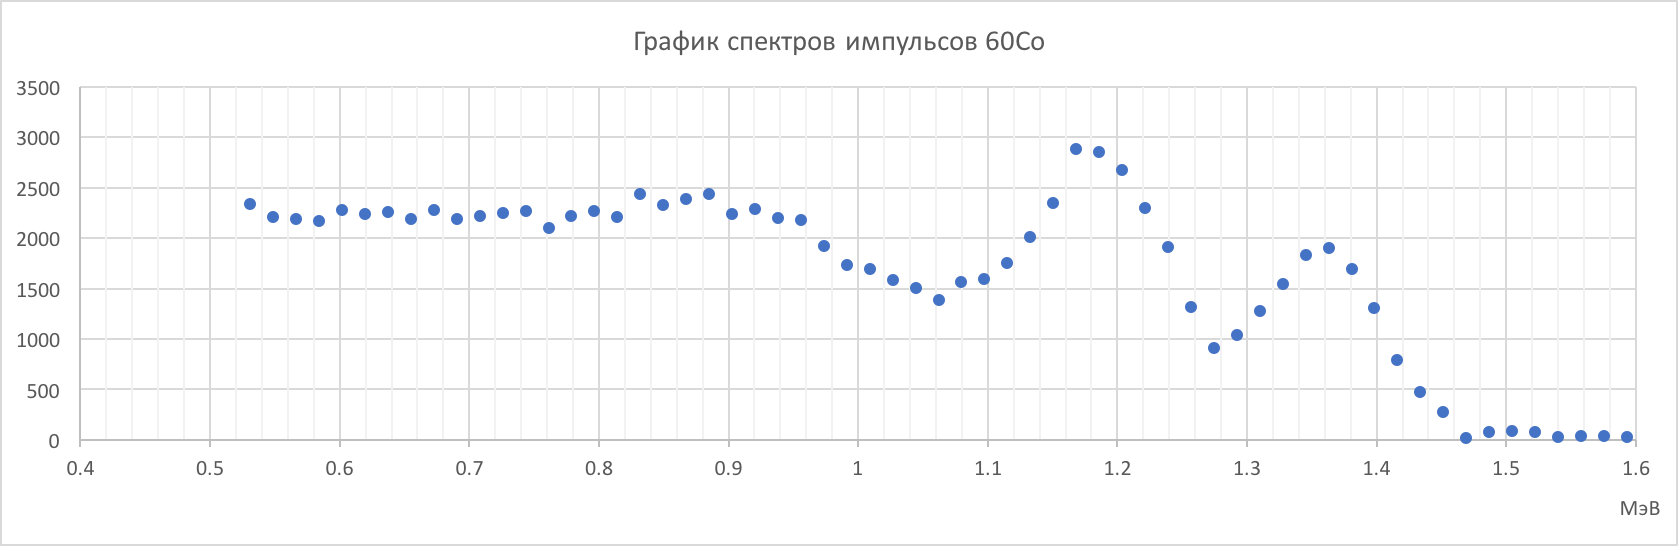
\includegraphics[width = \lw]{60Co}
    \caption{Графики спектра импульсов $^{60}Co$}
\end{figure}

\begin{figure}[H]
\centering
    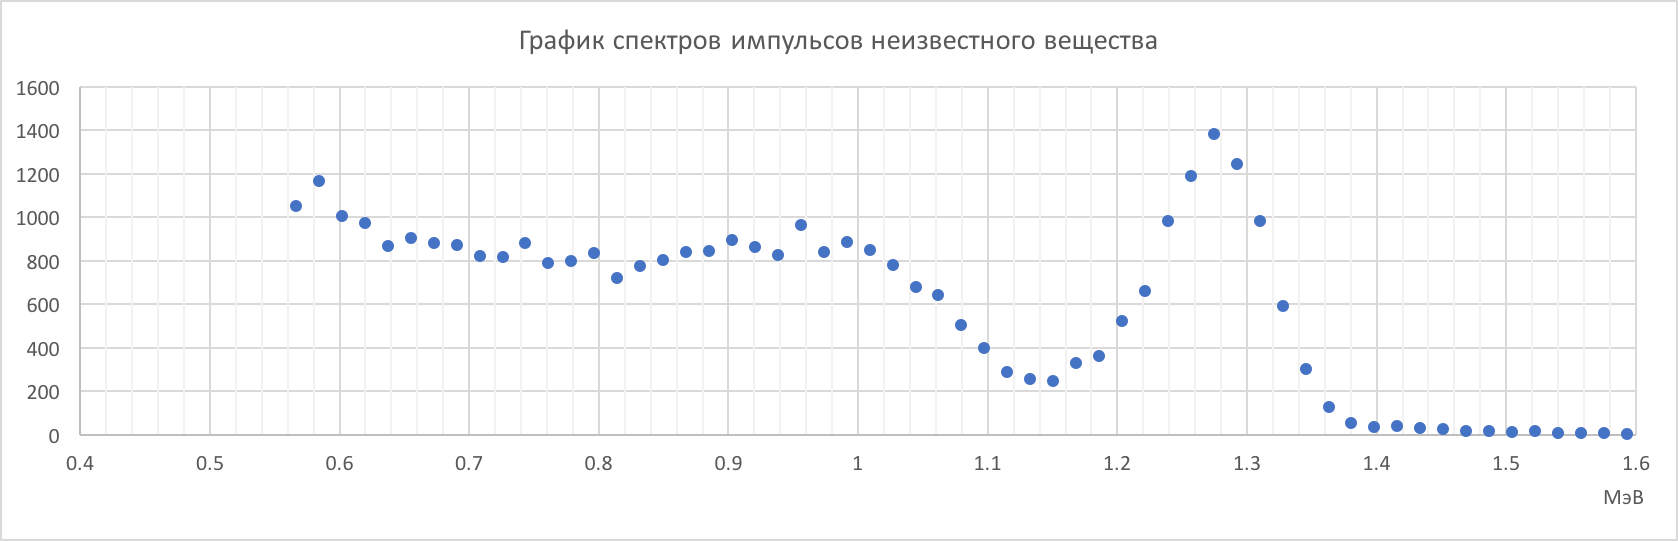
\includegraphics[width = \lw]{unknown}
    \caption{Графики спектра импульсов неизвестного вещества}
\end{figure}

По положению фотопиков определим энергию $\gamma$-квантов этого препарата. Зная энергию, посчитаем положение верхней границы комптоновского распределения и сравним с реальной экспериментальной величиной.

Энергия препарата $E_\gamma = 1.27 \pm 0.1$

Энергетическое разрешение прибора $R = \frac{\delta}{E_\gamma} \cdot 100 \% = 20 \%$

Верхняя граница комтоновского распределения: $(T_e)_{max} = 1.01~\M \eV$.

\section{Вывод}
Определили энергию $\gamma$-кванта неизвестного радиоактивного препарата после предварительно калибровки по $\gamma$-излучению $^{60}Co$. Посчитали энергетическое разрешение прибора, нашли положение верхней границы комптоновского распределения. 

\end{document}